\chapter{Tarea 1}

\framedt{Tarea a realizar}{

   Visualiza el siguiente vídeo:
   \href{
      https://www.youtube.com/watch?v=dEvtsZNrCSQ
   }{youtube.com/watch?v=dEvtsZNrCSQ}
   
   \begin{itemize}
   	\item Identifica en el sistema de distribución de agua los componentes físicos, ciberfísicos, y ciber
	\item Identifica los tipos de ataque que se describen en el vídeo, y explica brevemente como piensas que se podrían implementar.
	\item Explica cómo se plantea en el vídeo la defensa frente a los posibles ataques.
   \end{itemize}
}


\section{Componentes del sistema de distribución de agua}

\begin{paracol}{2}
   
\begin{itemize}
   \item \textbf{Componentes físicos:}
   \begin{itemize}
      \item Reservoirs
      \item Tanks
      \item Valves
      \item Pipes
      \item Pumps
      \item Taps in houses
   \end{itemize}
   \item \textbf{Componentes ciberfísicos:}
   \begin{itemize}
      \item Sensors
      \begin{itemize}
         \item Water temperature
         \item Water pressure
      \end{itemize}
      \item Logic Controllers (PLCs) que, por ejemplo,\\ pueden activar una valvula si una cisterna está casi vacía 
      \item Actuators in general
   \end{itemize}
   \item \textbf{Componentes ciber:}
   \begin{itemize}
      \item \textsc{Scada} (Supervisory Control and Data Acquisition)
      \item HMIs
      \item Networks
      \item Computadoras
   \end{itemize}
\end{itemize}
\switchcolumn
\colfill
\begin{figure}[htbp]
   \centering
   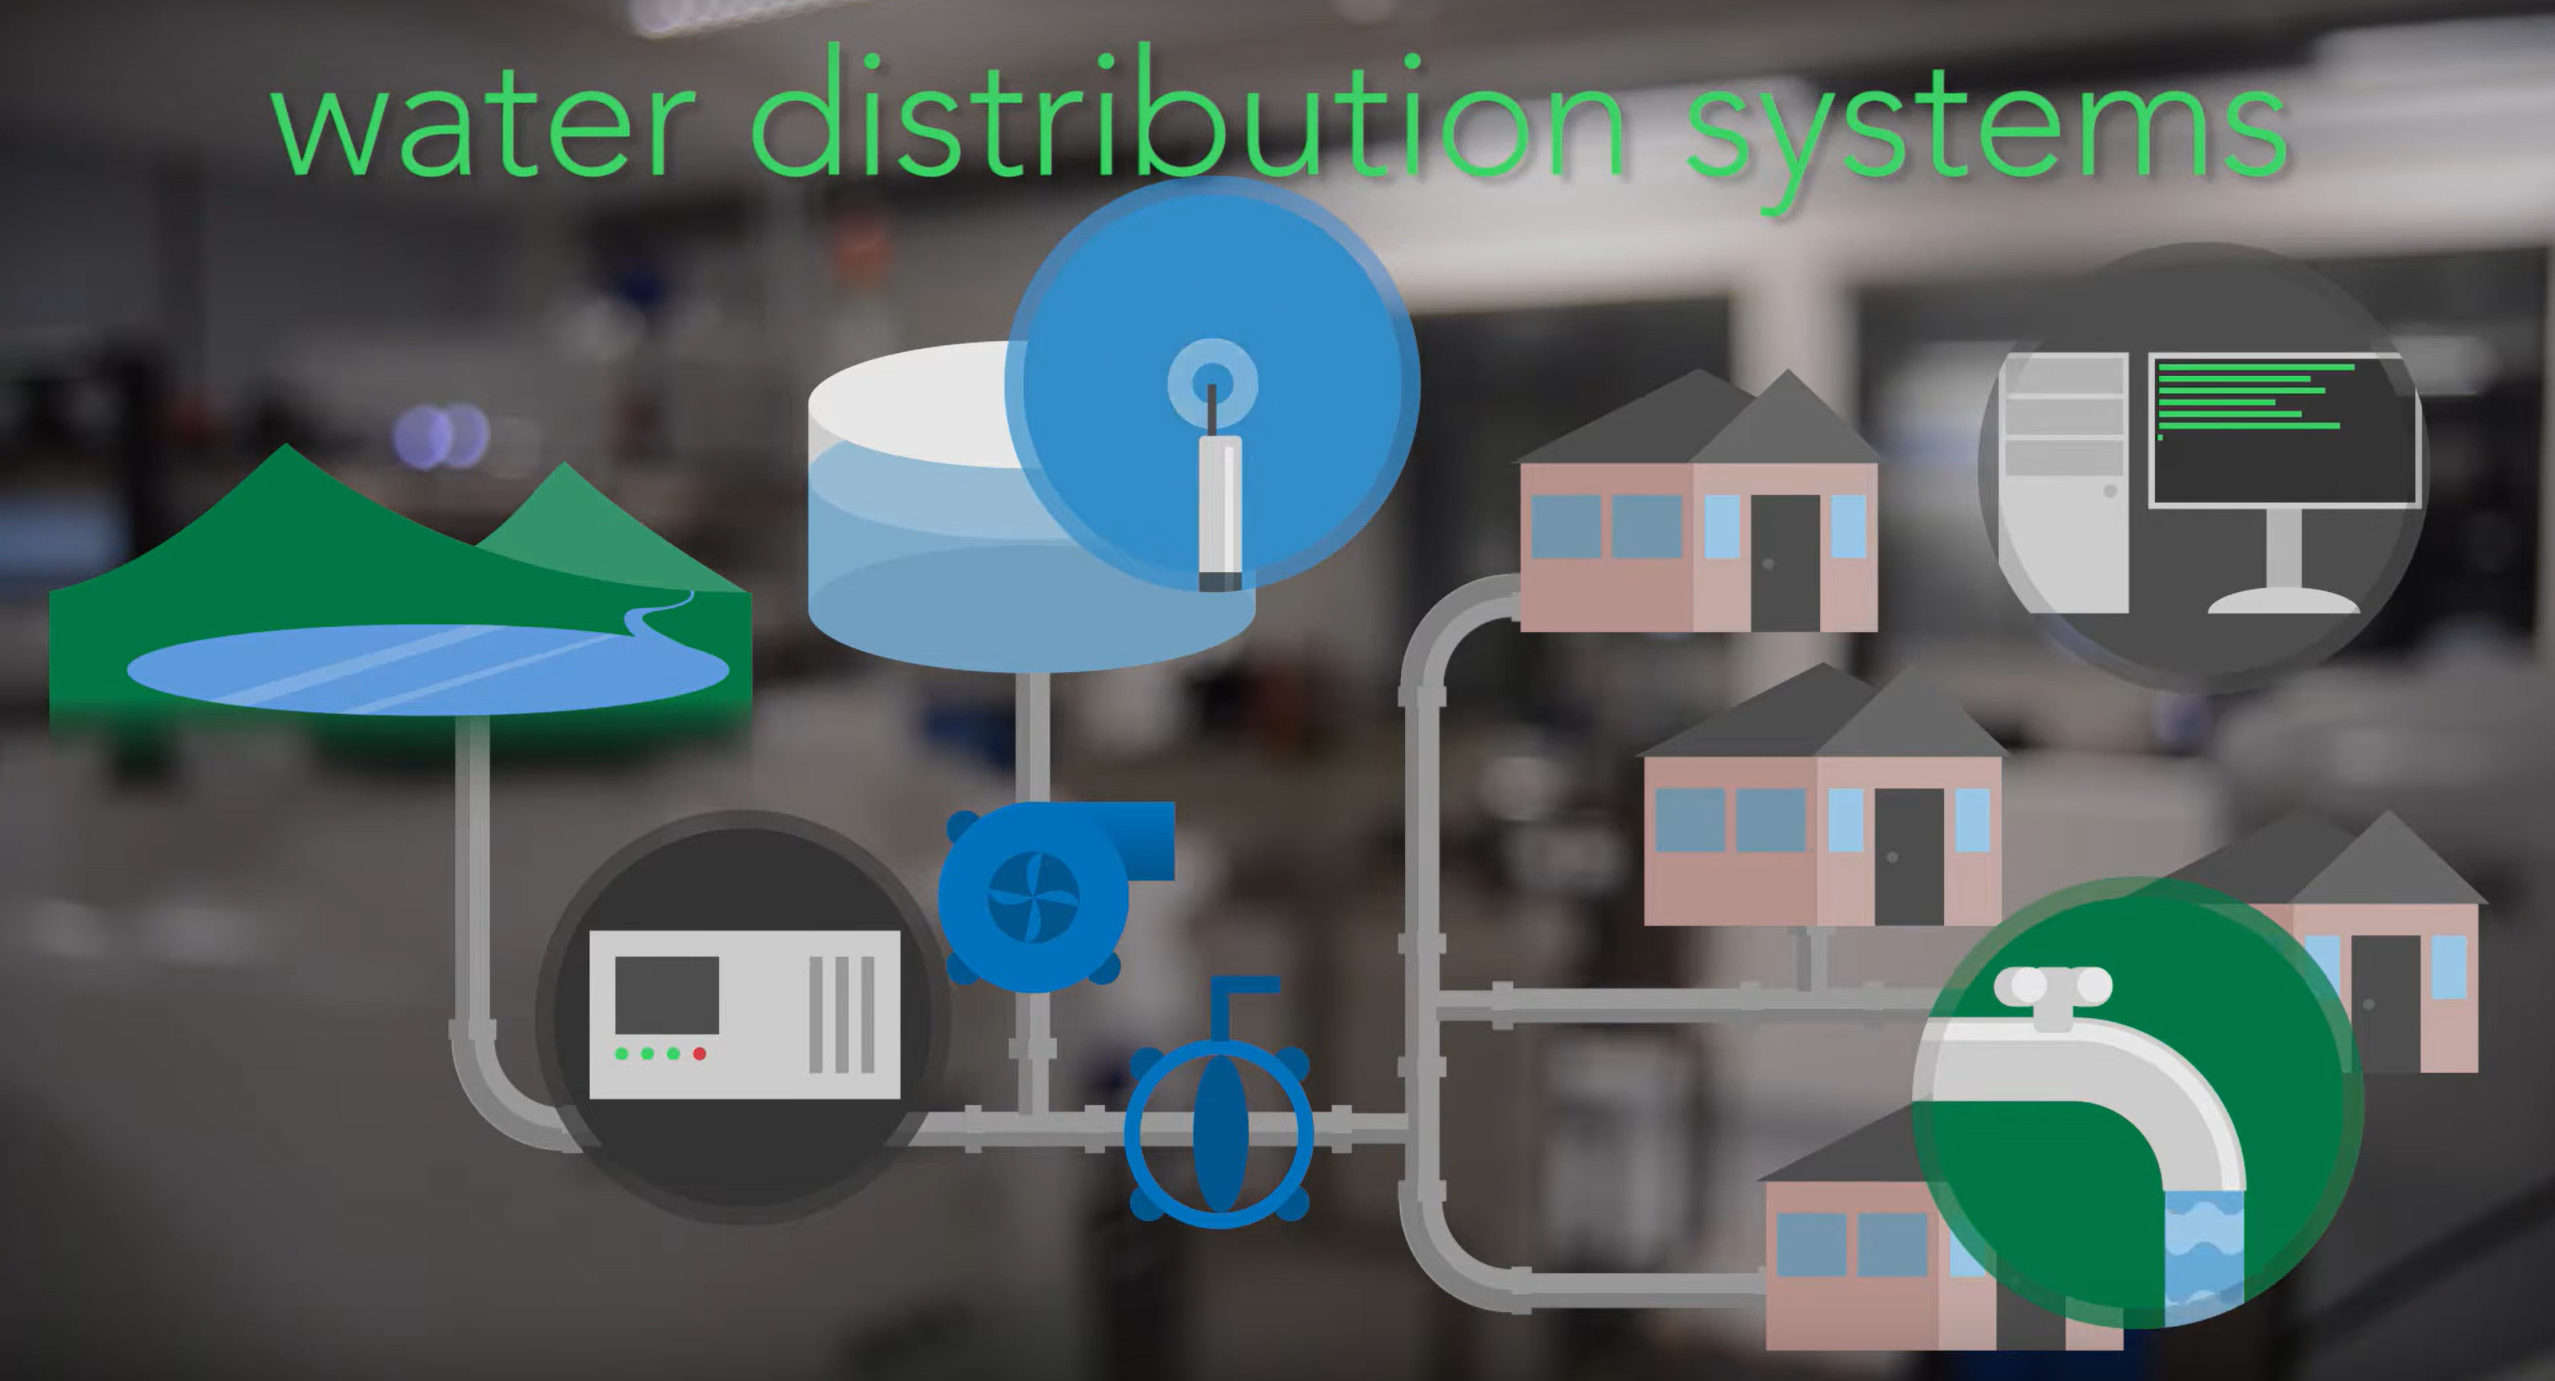
\includegraphics[width=0.95\columnwidth]{images/aguadistribucion.png}
   \caption{Esquema de un sistema de distribución de agua}
   \label{fig:aguadistribucion}
\end{figure}
\colfill

\end{paracol}

\section{Tipos de ataque}
Los componentes de sistemas ciberfísicos a menudo no implementan medidas de seguridad fuertes, convirtiéndolos en objetivo para atacantes, que pueden obtener acceso inicial a un sistema explotando sus vulnerabilidades.     
\begin{itemize}[itemsep=0.5em]
   \item \textbf{\ul{Robo de datos (Stealing data):}} Podrían implementarse mediante la infiltración en los sistemas \textsc{Scada} para extraer información confidencial sobre la infraestructura, patrones de uso, o datos de clientes. Esto podría realizarse mediante malware especializado o aprovechando vulnerabilidades en el software de control. Es posible también a traves de \textbf{packet sniffing}.
   
   \item \textbf{\ul{Daño al equipamiento (Damaging equipment):}} Manipulación de PLCs para operar bombas fuera de sus límites operativos. Similar al ataque Stuxnet que dañó centrifugadoras en Irán modificando frecuencias de operación.\\
   A veces, los sistemas empotrados no tienen \textbf{separación de privilegios} (monolithic kernel, todas las aplicaciones tienen el mismo ---máximo--- privilegio, falta de memory protection), lo que facilita la manipulación.
   
   \item \textbf{\ul{Corte del suministro de agua (Cutting off water supply):}} Cierre de válvulas o apagado de bombas mediante acceso no autorizado a \textsc{HMI}s (Human-Machine Interfaces);
   \textbf{command injection} ataques juntos a falta de \textbf{input validation} pueden permitir a un atacante ejecutar comandos arbitrarios en el sistema.
   
   \item \textbf{\ul{Liberación de sustancias tóxicas (Releasing toxic chemicals):}} Alteración de sistemas de dosificación química explotando {\textsc{PLC}}s con vulnerabilidades conocidas.\\
   Hemos mencionado en clase ``\textbf{Maroochy Shire}'', donde un ex-empleado de la empresa de control de aguas trató de liberar aguas residuales en el sistema de distribución, a través de un laptop y de una transmisión de radio para manipular bombas y válvulas.
   
   \item \textbf{\ul{Ataques de interceptación (Eavesdropping attacks):}} Captura de tráfico no cifrado entre sensores y controladores mediante herramientas como \textit{Wireshark}. Hemos visto que si pueden {alterar las funciones} de los protocolos \textsc{Scada} \textsc{Modbus} y \textsc{Dnp3} con fines malévolos. Además, \textsc{Scada} protocolos pueden carecer de \textbf{encriptación}, y, en cualquier caso, existen técnicas de \textit{Deep Packet Inspection} (\textsc{DPI}) que permiten deducir información incluso de paquetes cifrados.\\
   Una práctica comun es el \textbf{ARP spoofing} para redirigir el tráfico a un dispositivo de escucha.
   
   \item \textbf{\ul{Denegación de servicio (DoS):}} Saturación de interfaces de red de controladores \textsc{RTU/PLC}, o explotación de vulnerabilidades para inhabilitar dispositivos. Ejemplos típicos incluyen \textsc{syn} \textbf{flooding}, \textbf{Malformed packets injection} o \textbf{Smurf} ataques.
   
   \item \textbf{\ul{Ataques de engaño (Deception attacks):}} Falsificación de lecturas de sensores mediante ataques man-in-the-middle en protocolos vulnerables como OPC UA.\\
   El ataque a una \textit{Ukrainian Power Grid} en 2015 utilizó técnicas de engaño para hacer que los empleados obtuvieran un malware a través de correos electrónicos para comprometer la red.
\end{itemize}

Parte de estos ataques van a mostrar efectos evidentes en el sistema de distribución, pero los atacantes también pueden cubrir sus huellas manipulando los datos que se envían al sistema de control, engañando potencialmente tanto a humanos como a algoritmos.

\section{Defensa frente a ataques}

\begin{paracol}{2}
   \colfill
   La mejor defensa para \textit{Water Distribution Networks} es la \textbf{simulación de ataques}, sin embargo, actualmente no existe un método estándar para hacerlo.
   ``Attack models'' son modelos matemáticos que simulan los posibles comportamientos de un atacante.
   El video muestra \texttt{epanetCPA} es una herramienta que funciona en MATLAB que permite, dado un modelo de ataque, de ejecutar el modelo en una red \textsc{Epanet} (open-source toolkit para modelar y simular redes de distribución de agua), que es un modelo industrial estandar de red de agua, y ver cómo se comporta el sistema.\\
   Se puede controlar tanto el \textit{estado físico} del sistema como el \textit{estado cibernético} emulado del sistema, así que se puede \textbf{comparar} el comportamiento del sistema real con el comportamiento del sistema simulado.
   \colfill
   \switchcolumn

   \begin{figure}[htbp]
      \centering
      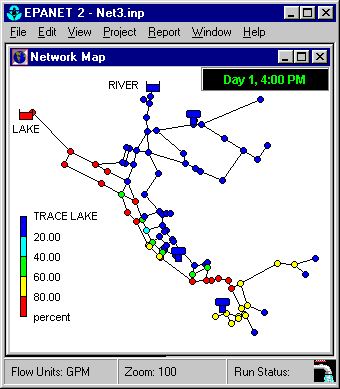
\includegraphics{images/EPANET-8.png}
      \caption{EPANET 2.0}
      \label{fig:EPANET}
   \end{figure}
\end{paracol}
   Tras un estudio, se observó que ataques a distintos componentes conducen a resultados similares, entonces encontrar un comportamiento anomalo en el sistema puede ser \textit{insuficiente} para determinar cual componente ha sido atacado, lo que hace necesaria una evaluación humana más completa.